\chapter{Fundamentos e Revisão de Literatura}

%-------------------------------------------------------------------
Este capítulo destina-se à definição de conceitos teóricos sobre as ferramentas e paradigmas utilizados no trabalho, os quais são listados a seguir: \emph{Framework Apache Hadoop}, \emph{MapReduce}, bem como trabalhos relacionados.

%-------------------------------------------------------------------
\section{Hadoop}
A origem do \emph{framework Apache Hadoop}, vem de outro projeto da \emph{Apache} \cite{Apache}, o \emph{Apache Nutch} \cite{Nutch}, que era um motor de buscas na \emph{web} com código livre iniciado em 2002. Porém o projeto encontrava problemas devido a sua arquitetura. Em 2003 quando a \emph{Google} publicou um artigo descrevendo a arquitetura utilizado no seu sistema de arquivos distribuídos, chamado GFS, os desenvolvedores viram que uma arquitetura semelhante resolveria o problema de escalabilidade do \emph{Nutch}.

Em 2004 os desenvolvedores do \emph{Nutch} começaram a implementar a ideia e o resultado foi nomeado \emph{Nutch Distributed Filesystem} (NDFS). A medida que o projeto avançava ele foi tomando proporções cada vez maiores, até que em 2006 foi criado um novo projeto pois os avanços já ultrapassavam o propósito do \emph{Nutch}, o novo projeto foi nomeado \emph{Hadoop}. O \emph{framework Hadoop} tem o propósito de facilitar o processamento distribuído através do paradigma do \emph{MapReduce}.

\subsection{Arquitetura geral do \emph{Apache Hadoop}}
De maneira geral é possível separar o \emph{Apache Hadoop} em duas partes, as quais são denominadas \emph{HDFS (Hadoop Distributed File System)} e \emph{YARN (Yet Another Resource Negotiator)}. A Figura \ref{fig:ArqGeral} fornece uma visão de como o \emph{framework} é estruturado.

\begin{figure}[hbtn]
   \centering
   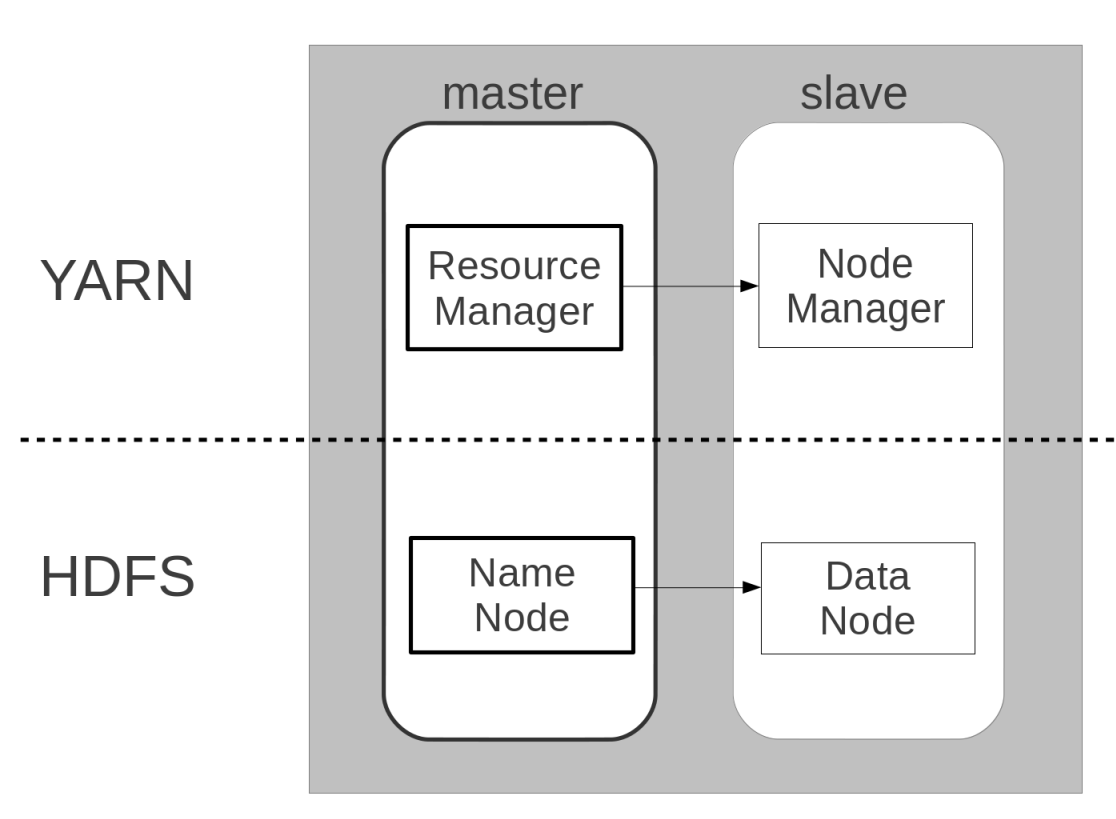
\includegraphics[width=9cm]{figuras/Figura08-HadoooArchGeral.png}
   \caption{Arquitetura geral do \emph{Apache Hadoop}}
   \label{fig:ArqGeral}
\end{figure}

O HDFS é a parte responsável pelo armazenamento dos dados necessários para que os jobs sejam executados, em outras palavras, é um grande HD distribuído como indica sua denominação (\emph{Distributed File System}). O HDFS é o componente que irá fazer a replicação de tolerância a falhas, distribuição dos dados de acordo com o que cada nó irá processar, entre outras atribuições.

A outra metade do \emph{Apache Hadoop}, o YARN, é responsável pelo processamento dos \emph{jobs} submetidos ao \emph{cluster}. É dentro do YARN que as tarefas de \emph{MapReduce} são executadas, consequentemente o YARN é o componente que gerencia todos os recursos do \emph{cluster}. 

\subsubsection{HDFS}
O HDFS é em grande parte responsável pelo bom desempenho do \emph{Apache Hadoop}, pois é encarregado com a tarefa de não sobrecarregar a rede com transferência de arquivos. No HDFS o acesso a arquivo é sempre local, isso quer dizer que cada nó receberá a parte do arquivo referente a sua carga de trabalho, evitando assim replicação desnecessária além da básica para segurança e tolerância a falhas.
Um problema dessa abordagem é que o \emph{Hadoop} possui uma latência muito alta, sendo desaconselhável o uso do \emph{Hadoop} em aplicações críticas ou de tempo real. O HDFS pode ser subdivido em dois serviços, \emph{NameNode} e \emph{DataNode}, responsáveis pelo gerenciamento dos dados a nível de \emph{cluster} e gerenciamento dos dados a nível local, respectivamente. A Figura \ref{fig:ArqHDFS} apresenta um esquema básico da arquitetura do HDFS.

\begin{figure}[hbtn]
   \centering
   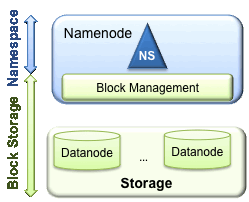
\includegraphics[width=8cm]{figuras/Figura07-HDFS.png}
   \caption{Arquitetura geral do HDFS \cite{HDFS}}
   \label{fig:ArqHDFS}
\end{figure}

\subsubsection{YARN}
O YARN é a parte do \emph{Apache Hadoop} responsável pela execução do \emph{MapReduce}, portanto à ele cabem as tarefas de gerenciamento e execução do processamento. Ao tornar a tarefa de processamento totalmente independente das tarefas de armazenamento, o \emph{Apache Hadoop} abre muitas possibilidades para sua utilização. Assim como o HDFS, o YARN pode ser subdividido em 2 serviços, \emph{ResourceManager} e \emph{NodeManager}, responsáveis pelo gerenciamento dos recursos no sistema e pelo gerenciamento dos recursos locais, respectivamente. A Figura \ref{fig:ArqYARN} apresenta um esquema básico da arquitetura do YARN.

\begin{figure}[hbtn]
   \centering
   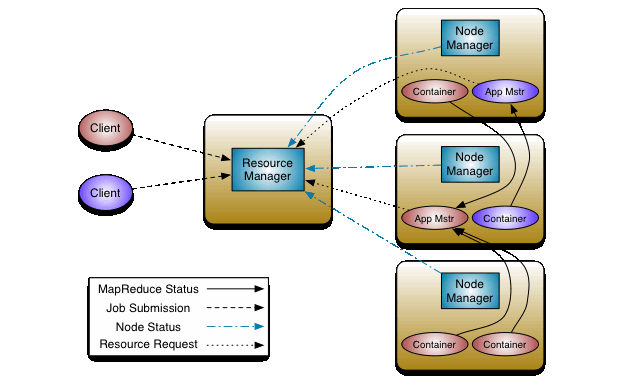
\includegraphics[width=12cm]{figuras/Figura06-YarnArch.png}
   \caption{Arquitetura geral do YARN \cite{YARN}}
   \label{fig:ArqYARN}
\end{figure}

Embora não demonstrado na imagem, cada serviço possui diversos módulos internos, por exemplo o \emph{ResourceManager} possui o Escalonador e o \emph{ApplicationsManager}, os quais ainda podem ser divididos em sub-módulos menores. O presente trabalho busca apresentar uma nova solução para a maneira de escalonamento empregada no \emph{Hadoop} que se adapte melhor ao ambiente.

\subsection{Configuração do ambiente de execução do \emph{Hadoop}}
Um ambiente corretamente configurado do \emph{Hadoop} possui alguns pré-requisitos além dos nós acessíveis entre si em uma rede. Cada nó deve ter em sua instalação do \emph{Hadoop} vários arquivos xml, que são responsáveis pela configuração das MVs do \emph{Hadoop} naquela máquina.
Para conhecimento, esses arquivos são: \emph{core-site.xml, yarn-site.xml, mapred-site.xml} e \emph{hdfs-site.xml}. Cada um desses arquivos terá a configuração de um serviço do \emph{Hadoop}. O arquivo \emph{hdfs-site.xml} por exemplo é responsável pela configuração do HDFS naquela máquina.
É importante salientar que esta configuração em nenhum momento é realizada automaticamente pelo \emph{Hadoop} e que o usuário deve configurar cada nó separadamente.

%%incluir apendices/anexos com as configurações utilizadas?

\subsection{\emph{MapReduce}}
O paradigma de \emph{MapReduce}, já citado várias vezes no presente trabalho, divide o processamento em duas etapas. Essas duas etapas são derivadas das funções \emph{Map} e \emph{Reduce} das linguagens funcionais, e assim como nas funções oiginais, elas tem funcionamento baseado em tuplas de chave e valor. Um ciclo de aplicação típico é a função \emph{Map} receber um arquivo de entrada e buscar os valores procurados pela aplicação, então formar tuplas de chave e valor. Feitas as tuplas, a função \emph{Map} manda o resultado para a \emph{Reduce} onde as chaves serão processadas e reduzidas a dados mais significativos. A grande vantagem do \emph{Hadoop} é que dado um ambiente corretamente configurado, o programador pode focar sua atenção à resolução das tarefas pelo paradigma do \emph{MapReduce} e não em como o trabalho será distribuído.

\section{Sensibilidade ao contexto}
Dada a interligação dos sistemas hoje em dia, já é possível notar alguma sensibilidade ao contexto na maioria deles. Ao acessar um site por um dispositivo móvel, o site automaticamente irá carregar sua versão \emph{mobile}, a qual foi projetada para estes dispositivos, ou quando os navegadores utilizam dados de localidade para oferecer produtos, entre outros exemplos de utilização do contexto.

Segundo \cite{Zakaria}, sensibilidade ao contexto na computação se refere a habilidade de uma aplicação de detectar e responder as mudanças no ambiente de execução. O que leva a seguinte definição feita por \cite{Baldauf}, onde ele afirma que um sistema sensível ao contexto é capaz de adaptar suas operações ao contexto atual sem intervenção explicita do usuário e portanto aumentar sua usabilidade e eficácia.

Partindo dessas duas afirmações vem a dúvida sobre o que seria o contexto, portanto a definição do contexto é fundamental para que haja um entendimento da sensibilidade ao contexto \cite{Manuele}. O contexto pode assumir diversos significados dependendo da situação que se encontra, \cite{Dey} define contexto como qualquer informação que pode ser utilizada para caracterizar a situação de uma entidade (pessoa, lugar ou objeto) considerado relevante para a interação entre usuário e aplicação.

Geralmente informações de contexto são utilizadas para a melhoria de performance de um sistema ou algoritmo, portanto estima-se ser possível melhorar a execução do \emph{Apache Hadoop} através da utilização dessa técnica. 

Embora existam diversas maneiras de se utilizar essas informações de contexto para melhorar a performance do \emph{MapReduce}, \cite{Manuele} cita três exemplos de como isso pode ser feito, os quais se resumem em: configuração automática dos nós durante a instalação, gerenciamento de entrada e saída de nós do \emph{cluster} e finalmente na distribuição de tarefas feita pelo escalonador de acordo com a disponibilidade de recursos e tarefas já em execução. A terceira maneira apresentada é a maneira que corresponde à abordagem utilizada nesse trabalho.

\section{Escalonadores para Hadoop}
Uma dos principais componentes do \emph{Hadoop} é o escalonador, componente responsável pela distribuição do trabalho no ambiente. Além dos escalonadores disponibilizados juntamente com o próprio \emph{Hadoop}, existem outras implementações que buscam solucionar uma necessidade específica que os escalonadores padrões não oferecem suporte.

\subsection{\emph{Hadoop Internal Scheduler}}
O escalonador padrao do \emph{Hadoop} foi implementado visando suportar apenas a submissão de tarefas em lote. Nesse escalonador, a primeira tarefa recebida é a primeira executada, formando uma fila para as subsequentes. Apesar de simples este escalonador também suporta cinco níveis de prioridade, porém a escolha da próxima tarefa nunca deixará o tempo de submissão completamente de fora.

\subsection{\emph{Fair Scheduler}}
Utilizado para computar tarefas pequenas em lote que possuam os mesmos dados de entrada, utilizando um escalonamento em dois níveis para distribuir recursos igualitáriamente \cite{FairScheduler}. O nível superior, geralmente aloca filas para cada usuário, utilizando um algoritmo justo com pesos. O segundo nível aloca os recursos dentro de cada fila, e utiliza um algoritmo igual ao \emph{Internal Scheduler}.

\subsection{\emph{Capacity Scheduler}}
Este escalonador surgiu para os casos onde um ambiente \emph{Hadoop} é dividido entre várias empresas ou possui partes distribuídas em diversos locais sob responsabilidade de mais de um dono. Ele é focado em garantias de que uma quantidade mínima de recursos será disponibilizada a qualquer momento que um de seus usuários decidir utilizar o \emph{Hadoop}. O benefício decorre que organizações diferentes possuem picos de processamento em horas diferentes, portanto as organizações que estão utilizando o \emph{Hadoop} irão se aproveitar da capacidade ociosa das outras.

\section{Trabalhos relacionados}

Foi feita uma pesquisa bibliográfica com objetivo de analisar os trabalhos que já haviam sido desenvolvidos envolvendo o \emph{Hadoop} e que se propunham a alterar ou adaptar o escalonador. Além disso, buscou-se identificar quais técnicas eram as mais utilizadas e em cima de quais objetivos o trabalho foi desenvolvido. A seguir encontram-se os trabalhos relacionados e um breve resumo sobre a proposta, contexto utilizado e objetivo esperado com as alterações.

\begin{itemize}
\item CASH (\emph{Context Aware Scheduler for Hadoop}) \cite{CASH}, nesse trabalho o objetivo dos autores é de melhorar o rendimento geral do \emph{cluster}. Eles partem da hipótese de que grande parte dos jobs são periódicos e executados no mesmo horário, além de possuírem características de uso de CPU, rede, disco etc. semelhantes. O trabalho ainda leva em consideração que com o passar do tempo os nós tendem a ficar mais heterogêneos. Com a intenção de solucionar esses problemas e baseados nessas hipóteses, foi implementado um escalonador que classifica tanto os jobs como as máquinas com relação ao seu potencial de CPU e E/S, podendo então distribuir os jobs para máquinas que tem uma configuração apropriada para sua natureza.

\item LATE (\emph{Longest Approximation Time to End}) \cite{LATE}, seguindo o que o nome sugere, nesse tabalho a informação de contexto é referente ao tempo estimado de término da \emph{task} baseado numa heurística que faz a relação de tempo decorrido e \emph{score}. Essa informação é usada também para gerar um limiar de quando uma \emph{task} é lenta o suficiente para indicar sitomas de erros e então iniciar uma nova em outra máquina possívelmente mais rápida. O objetivo do trabalho era de reduzir o tempo de resposta em \emph{clusters} grandes que executam muitos \emph{jobs} de pequena duração.

\item \emph{A Dynamic MapReduce Scheduler for Heterogeneous Workloads} \cite{DMRSHW}, aqui os autores também utilizam a técnica de classificar os \emph{jobs} e máquinas de acordo com a quantidade de E/S ou CPU. E assim como no CASH, o principal objetivo é a melhora de rendimento no \emph{cluster}. Uma das diferenças, no entanto, é que essa implementação utiliza um escalonador com três filas.

\item SAMR (\emph{A Self-adaptative MapReduce}) \cite{SAMR}, essa implementação segue a mesma ideia do LATE, onde a informação de contexto é referente ao cálculo do progresso de uma \emph{task} para identificar se é necessário lançar outra task igual ou não. Porém essa solução varia o cálculo do progresso de acordo com informações do ambiente em que a \emph{task} está sendo executada, seu principal objetivo é a redução do tempo de execução das \emph{tasks}. Para que sejam utilizadas informações do ambiente, o algoritmo leva em consideração informações históricas contidas em cada nó, e ajusta o peso de cada estágio do processamento.

\item COSHH (\emph{A Classification and Optimization based Scheduler for Heterogeneous Hadoop Systems}) \cite{COSHH}, um pouco mais abrangente das demais soluções apresentadas, essa solução leva em consideração informações não especificadas sobre o sistema. Seu ganho de performance se dá a partir da classificação dos \emph{jobs} em classes, ele então faz uma busca por máquinas que se encaixem nessa mesma classe. Essa busca é feita por um algoritmo que reduz o tamanho do espaço de busca para melhorar o rendimento. O objetivo dessa solução é a melhora do tempo médio em que os \emph{jobs} são completados, além de oferecer uma boa performance quando utilizando somente o fatia mínima, além de proporcionar uma distribuição justa.

\item \emph{Quincy} \cite{Quincy}, diferentemente de todos os outros trabalhos, essa solução não foi desenvolvida visando somente o \emph{Hadoop} mas ainda assim é aplicável ao mesmo. Possuindo como objetivo melhorar o desempenho geral de um \emph{cluster}, utiliza como informação de contexto a distribuição de recursos e modifica a maneira tradicional de tratamento desses. Ao utilizar um modo mais dinâmico do que o convencional, a solução mapeia os recursos num grafo de capacidades e demandas e calcula o escalonamento ótimo a partir de uma função global de custo.

\item \emph{Improving MapReduce Performance through Data Placement in heterogeneous Hadoop Clusters} \cite{IMRPDPHHC}, buscando melhorar a performance de \emph{jobs} que possuam muito processamento de dados através da melhor distribuição desses dados, essa solução utiliza principalmente a localidade dos dados como informação para tomada de decisões. O ganho de performance é dado pelo rebalanceamento dos dados nos nós, deixando nós mais rápidos com mais dados. Isso diminui o custo de \emph{jobs} especulativos e de transferência de dados pela rede.
\end{itemize}

Após estudo dos trabalhos, nota-se que muitos deles tem por objetivo a diminuição do tempo de resposta ou a melhoria do rendimento de maneira geral, os quais diferem dos objetivos do presente trabalho, que na verdade busca proporcionar uma melhor adaptação do \emph{Hadoop} a um ambiente heterogêneo. 

Constata-se também que há uma diversidade de contextos levados em consideração, contudo é possível identificar temas recorrentes como : a classificação dos \emph{jobs} e dos nós quanto ao potencial de E/S ou de CPU, a avaliação do progresso da \emph{task} na decisão de lançar ou não uma nova \emph{task} especulativa.